\documentclass{standalone}
\usepackage{tikz}
\usepackage{amsmath}
\usetikzlibrary{arrows.meta, positioning}

\begin{document}
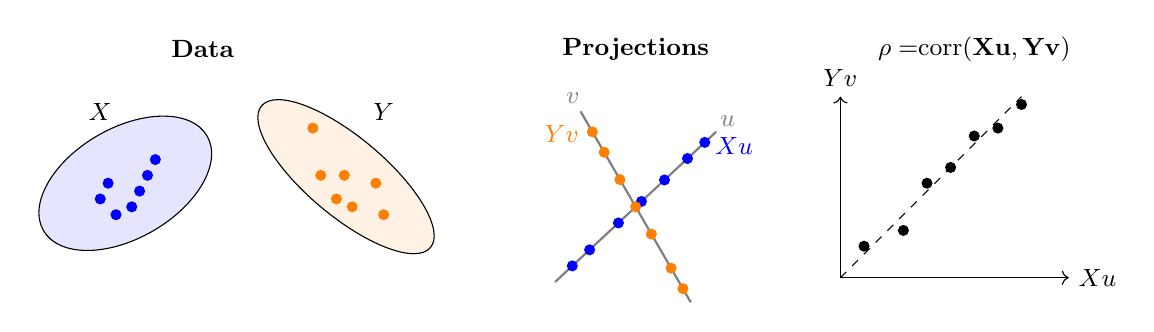
\begin{tikzpicture}[font=\small, every node/.style={font=\small}]

% Offsets for moving the clouds
\def\Xoffx{-2.4}
\def\Xoffy{0.1}

\def\Yoffx{0.4}
\def\Yoffy{0.2}

% --- Left Panel: Data clouds ---
\node at (-1.5,2.0) {\textbf{Data}};
% Ellipses
\draw[fill=blue!10,   rotate=30]  (-2,1.5) ellipse (1.2 and 0.7);
\draw[fill=orange!10, rotate=-40] (0,0.5)  ellipse (1.4 and 0.5);

% Dots in X (placed well inside the left ellipse)
\foreach \dx/\dy in {
   0.3/0.5,
   0.2/0.3,
  -0.4/0.0,
  -0.2/-0.2,
   0.1/0.1,
   0.0/-0.1,
  -0.3/0.2
}
  \fill[blue] ({\Xoffx+\dx},{\Xoffy+\dy}) circle (2pt);

% Draw Y points
\foreach \dx/\dy in {
  -0.5/0.8,
   0.4/-0.3,
  -0.4/0.2,
  -0.2/-0.1,
   0.3/0.1,
  -0.1/0.2,
   0.0/-0.2
}
  \fill[orange] ({\Yoffx+\dx},{\Yoffy+\dy}) circle (2pt);

% Labels X and Y
\node at (-2.8,1.2) {$X$};
\node at (0.8,1.2) {$Y$};


% --- Middle Panel: Projections ---
\begin{scope}[shift={(4,0)}]

  % Angles (in degrees)
  \def\angleu{43}
  \def\anglev{120}

  % Line u
  \draw[gray, thick]
    ({-1.4*cos(\angleu)},{-1.4*sin(\angleu)}) --
    ({ 1.4*cos(\angleu)},{ 1.4*sin(\angleu)});
  \node[gray] at ({1.6*cos(\angleu)},{1.6*sin(\angleu)}) {$u$};

  % Line v
  \draw[gray, thick]
    ({-1.4*cos(\anglev)},{-1.4*sin(\anglev)}) --
    ({ 1.4*cos(\anglev)},{ 1.4*sin(\anglev)});
  \node[gray] at ({1.6*cos(\anglev)},{1.6*sin(\anglev)}) {$v$};

  % 7 points on u (not equispaced)
  \foreach \t in {-1.1,-0.8,-0.3,0.1,0.5,0.9,1.2}
    \fill[blue] ({\t*cos(\angleu)},{\t*sin(\angleu)}) circle (2pt);
  \node[blue, above right]
    at ({0.8*cos(\angleu)+0.3},{0.8*sin(\angleu)}) {$Xu$};

  % 7 points on v (not equispaced)
  \foreach \t in {-1.2,-0.9,-0.4,0.0,0.4,0.8,1.1}
    \fill[orange] ({\t*cos(\anglev)},{\t*sin(\anglev)}) circle (2pt);
  \node[orange, above left]
    at ({0.8*cos(\anglev)-0.2},{0.8*sin(\anglev)}) {$Yv$};

  % Panel label
  \node at (0,2.0) {\textbf{Projections}};
\end{scope}

% --- Right Panel: Correlation scatter ---
\begin{scope}[shift={(7.5,0)}]
  % Axes
  \draw[->] (-0.9,-0.9) -- (2,-0.9) node[right] {$Xu$};
  \draw[->] (-0.9,-0.9) -- (-0.9,1.4) node[above] {$Yv$};

  % Scatter points
  \foreach \x/\y in {-0.6/-0.5, -0.1/-0.3, 0.2/0.3, 0.5/0.5, 0.8/0.9, 1.1/1.0, 1.4/1.3}
    \fill[black] (\x,\y) circle (2pt);

  % Regression line
  \draw[dashed] (-0.9,-0.9) -- (1.4,1.4);

  % Correlation label
    \node at (0.8,2.0) {$\mathbf{\rho =} \mathbf{\mathrm{corr}(Xu, Yv)}$};
\end{scope}

\end{tikzpicture}
\end{document}


